\subsection{Architecture Overview}

The MicroNet framework is a collection of components. Each component is
confined in itself which allows simple replacement of components. The components
are organized in three layers: The framework layer, the service catalogue layer,
and the tools layer. \autoref{fig:architecture_layers} shows the layers and the
components they contain.

\begin{figure}
  \centering
  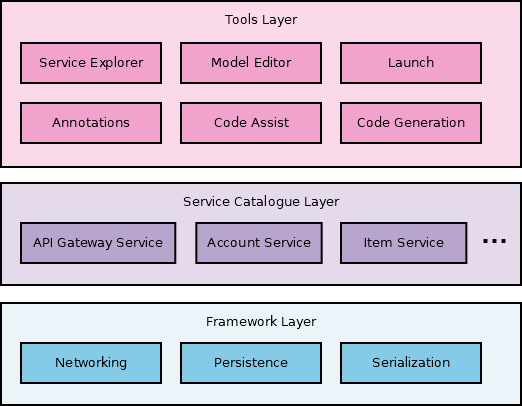
\includegraphics[width=0.7\textwidth]{images/architecture/ArchitectureLayers}
  \caption{The layered architecture of MicroNet with the associated components.}
  \label{fig:architecture_layers}
\end{figure}


The layers and the components they contain are explained below using Component
Responsibility Cards (CRC).

\newpage
\subsubsection{Framework Layer}

The framework layer provides a uniform interface to the core functionality of
MicroNet.\\

\begin{tabular}{|l|l|}
    \cline{1-2}
    \multicolumn{2}{|c|}{} \\[-0.3cm]
    \multicolumn{2}{|c|}{Networking Component} \\ 
    \multicolumn{2}{|c|}{} \\[-0.3cm]
    \cline{1-2}
    Responsibility & Collaboration \\
    \cline{1-2}
    & \\[-0.2cm]
    \begin{minipage}{6.5cm}
        \begin{itemize}
          \item Reliable Messaging System
          \item Connection Authentication
          \item Messaging API
        \end{itemize} 
    \end{minipage}
	&
    \begin{minipage}{6.5cm}
        \begin{itemize}
          \item Message Broker (ActiveMQ)
          \item Serialization Component
        \end{itemize} 
    \end{minipage}
	\\ & \\
    \hline
\end{tabular}

\vspace{0.5cm}

\begin{tabular}{|l|l|}
    \cline{1-2}
    \multicolumn{2}{|c|}{} \\[-0.3cm]
    \multicolumn{2}{|c|}{Persistence Component} \\ 
    \multicolumn{2}{|c|}{} \\[-0.3cm]
    \cline{1-2}
    Responsibility & Collaboration \\
    \cline{1-2}
    & \\[-0.2cm]
    \begin{minipage}{6.5cm}
        \begin{itemize}
          \item Uniform Database Access
          \item Offer Relational Database 
          \item Offer NoSQL Database
          \item Java API
        \end{itemize} 
    \end{minipage}
	&
    \begin{minipage}{6.5cm}
        \begin{itemize}
          \item Relational DBMS (PostgreSQL)
          \item JDBC
          \item NoSQL Database (Couchbase)
        \end{itemize} 
    \end{minipage}
	\\ & \\
    \hline
\end{tabular}

\vspace{0.5cm}

\begin{tabular}{|l|l|}
    \cline{1-2}
    \multicolumn{2}{|c|}{} \\[-0.3cm]
    \multicolumn{2}{|c|}{Serialization Component} \\ 
    \multicolumn{2}{|c|}{} \\[-0.3cm]
    \cline{1-2}
    Responsibility & Collaboration \\
    \cline{1-2}
    & \\[-0.2cm]
    \begin{minipage}{6.5cm}
        \begin{itemize}
          \item Uniform Serialization API
          \item Make serialization technology interchangeable
          \item Json serialization
          \item Binary serialization
        \end{itemize} 
    \end{minipage}
	&
    \begin{minipage}{6.5cm}
        \begin{itemize}
          \item Serialization Library (Gson)
        \end{itemize} 
    \end{minipage}
	\\ & \\
    \hline
\end{tabular}

\subsubsection{Service Catalogue Layer}

The service catalogue was a major topic in the second semester thesis
\todo{cite thesis 2}. This section will only give three examples of services.\\

\begin{tabular}{|l|l|}
    \cline{1-2}
    \multicolumn{2}{|c|}{} \\[-0.3cm]
    \multicolumn{2}{|c|}{API Gateway Service} \\ 
    \multicolumn{2}{|c|}{} \\[-0.3cm]
    \cline{1-2}
    Responsibility & Collaboration \\
    \cline{1-2}
    & \\[-0.2cm]
    \begin{minipage}{6.5cm}
        \begin{itemize}
          \item Receive and filter requests from clients
          \item Forward requests to \mss{}
          \item Forward Events to clients
          \item Broadcast events to groups of clients
        \end{itemize} 
    \end{minipage}
	&
    \begin{minipage}{6.5cm}
        \begin{itemize}
          \item Account Service (connection authentication)
        \end{itemize} 
    \end{minipage}
	\\ & \\
    \hline
\end{tabular}

\vspace{0.5cm}

\begin{tabular}{|l|l|}
    \cline{1-2}
    \multicolumn{2}{|c|}{} \\[-0.3cm]
    \multicolumn{2}{|c|}{Account Service} \\ 
    \multicolumn{2}{|c|}{} \\[-0.3cm]
    \cline{1-2}
    Responsibility & Collaboration \\
    \cline{1-2}
    & \\[-0.2cm]
    \begin{minipage}{6.5cm}
        \begin{itemize}
          \item User Registration
          \item User Authentication
        \end{itemize} 
    \end{minipage}
	&
    \begin{minipage}{6.5cm}
        \begin{itemize}
          \item Account Database (PostgreSQL)
        \end{itemize} 
    \end{minipage}
	\\ & \\
    \hline
\end{tabular}

\vspace{0.5cm}

\begin{tabular}{|l|l|}
    \cline{1-2}
    \multicolumn{2}{|c|}{} \\[-0.3cm]
    \multicolumn{2}{|c|}{Item Service} \\ 
    \multicolumn{2}{|c|}{} \\[-0.3cm]
    \cline{1-2}
    Responsibility & Collaboration \\
    \cline{1-2}
    & \\[-0.2cm]
    \begin{minipage}{6.5cm}
        \begin{itemize}
          \item Player Inventory (Carried Items)
          \item Bank (Item Storage)
        \end{itemize} 
    \end{minipage}
	&
    \begin{minipage}{6.5cm}
        \begin{itemize}
          \item Item Database (PostgreSQL)
        \end{itemize} 
    \end{minipage}
	\\ & \\
    \hline
\end{tabular}

\subsubsection{Tools Layer}

The development of the tool layer was a major part of this thesis. At a first
glance the tool layer's main purpose is to provide aid with the tenet
decentralized continuous delivery. But the tools layer has also the
responsibility to allow \ms{} application development in a way that is suitable
for \og{} development.\\

\begin{tabular}{|l|l|}
    \cline{1-2}
    \multicolumn{2}{|c|}{} \\[-0.3cm]
    \multicolumn{2}{|c|}{Annotation Processing} \\ 
    \multicolumn{2}{|c|}{} \\[-0.3cm]
    \cline{1-2}
    Responsibility & Collaboration \\
    \cline{1-2}
    & \\[-0.2cm]
    \begin{minipage}{6.5cm}
        \begin{itemize}
          \item Framework functionality\footnotemark 
          \item Boilerplate code reduction
          \item Defining the shared messaging API
        \end{itemize} 
    \end{minipage}
	&
    \begin{minipage}{6.5cm}
        \begin{itemize}
          \item Account Database (PostgreSQL)
        \end{itemize} 
    \end{minipage}
	\\ & \\
    \hline
\end{tabular}

\footnotetext{The user code is
          called by the framework (application skeleton) opposed to the user
          code calling a library (well-defined operations).}
